\chapter{AQUISIÇÃO DE DADOS E DEPENDÊNCIAS}
    
    Neste capítulo será discutido como é realizada a aquisição de dados MT, e quais as técnicas atualmente utilizadas para o processamento dos dados. Também será mostrado quais as dependências que foram necessárias para a construção do \software, dentre elas estão: Kivy, EMTF (Dnff e TranMT) e conversores de dados.
        
    \section{Aquisição de Dados MT}        
    
        A aquisição de dados MT consiste na obtenção dos campos elétricos ($\campo{E}_x$ e $\campo{E}_y$) e magnéticos através dos campos magnetizantes ($\campo{H}_x$, $\campo{H}_y$ e $\campo{H}_z$), onde são os parâmetros essenciais para o cálculo da impedância ($Z$), equações \ref{EZHvetor} e \ref{tensor-impe}.
        
        Devido a sensibilidade do sinal das sondagens MT, os sensores devem proporcionar uma alta relação sinal/ruído e alta capacidade de ampliar o sinal medido.
        
        O arranjo amplamente adotado para aquisição, são três magnetômetros distribuídos cada um paralelo a um eixo cartesiano, responsáveis pelos campos magnéticos. Para os campos elétricos, são distribuídos dois arranjos de eletrodos não polarizados, onde são acoplados horizontalmente, no sentido $x$ e $y$. A figura \ref{fig-arranjo-mt} mostra a disposição dos sensores na superfícies.
        
        Vale ressaltar que o eixo $x$ da composição cartesiana deve estar paralelo a direção do fluxo magnético terrestre, ou seja, direcionado ao polo geomagnético terrestre\footnote{Ponto na superfícies terrestre, onde, a inclinação magnética do modelo matemático para o campo magnético é $+90^\circ$}. 
        
        \begin{figure}[H]
            \caption{Arranjo para Aquisição de dados MT.}
                \begin{center}
                    \includegraphics[width=10cm]{texto/figura/arranjo-mt.eps}
                \end{center}
            \legend{\Fonte{\oautor.}}
            \label{fig-arranjo-mt}
        \end{figure}
        
        Os sensores registram a variação da amplitude do sinal em função do tempo, esses registros são chamados de series temporais e são considerados os dados brutos do método (Figura \ref{serie-temporal}).
        
        \begin{figure}[H]
            \caption{Exemplo de Série Temporal dos Dados MT.}
                \begin{center}
                    \includegraphics[width=16cm]{texto/figura/bor604a091_04D.pdf}
                \end{center}
            \legend{\Fonte{\oautor.}}
            \label{serie-temporal}
        \end{figure}
        
        Devido ao grande intervalo do espectro eletromagnético que abrange as sondagens MT ($10^{-4}\, Hz$ a $10^{4}\, Hz$), são configuradas varias taxas de aquisições diferentes. Para cada escolha de taxa de aquisição é considerada a representatividade do sinal respeitando a frequência de Nyquist \cite{nyquist28}. A representatividade é muito importante, pois, o sinal medido pelos sensores é a composição de várias ondas com frequências angulares diferentes, se a taxa de aquisição for menor que duas vezes a frequência da onda, ela não pode ser representada fielmente.  
        
        A Figura \ref{fig-aquisicao} exemplifica o conceito apresentado no paragrafo anterior, no exemplo é mostrado a composição de um onda com 10 frequências diferentes ($f_{\omega(t)}$), variando de $1$ a $10\, Hz$, se atribuirmos à ela uma taxa de aquisição de $10\,Hz$ pode-se perceber que a frequência de $6\,Hz$ não é representada corretamento, já percebe-se que para a frequência de $1\,Hz$ é super representada, isso acaba aumentando o tamanho dos arquivos de aquisição. A escolha da taxa de aquisição deve conciliar na melhor forma possível esses dois fatos.
        
        \begin{figure}[H]
            \caption{Aquisição de Dados Discretos.}
                \begin{center}
                    \includegraphics[width=13cm]{texto/figura/fourier2.eps}
                \end{center}
            \legend{\Fonte{\oautor.}}
            \label{fig-aquisicao}
        \end{figure}
    
        As taxas de aquisições comumente utilizadas são valores estimados por potências de 2, isso facilita na decomposição das frequências pela transformada de Fourier. Cada taxa de aquisição é chamada de \en{Banda} e varia de nome para cada equipamento utilizado. 
    
    \section{Processamento de Dados MT}
        Tradicionalmente o grande processamento de dados geofísicos é chamado de inversão, onde esse tenta ajustar um modelo físico que melhor represente o conjunto de dados. Porém para dados MT faz-se necessário antes das técnicas de inversão, o pré-processamento.
        
        O pré-processamento consiste, sucintamente, em realizar processamentos de filtragem, tratamentos estatísticos, conversão de dados, mudança de domínios e mesclagem de arquivos.
    
        A primeira etapa do pré-processamento é a conversão dos arquivos de binários para ASCII, esse processo é opcional, porem como boa prática é realizado para melhorar a legibilidade por parte dos usuários sobre os dados.
        
        Após a conversão são realizados técnicas de filtragem, a mudança do domínio dos dados de tempo para frequência angular, e cálculo do tensor impedância ($Z$). Esse processo será demonstrado mais detalhadamente no seção \ref{sec-robusto}, cuja a técnica recebe o nome de processamento Robusto, EMTF \cite{robusto-egbert}. Atualmente é a técnica mais confiável e amplamente utilizadas no meio acadêmico para tratamento dos dados.
        
        Como comentado na seção anterior, devido as limitações dos equipamentos, os dados são coletados separadamente para cada banda. Utilizando o processamento Robusto, esse gera um arquivo com extensão \en{.zss}. Nesses arquivos estão armazenados os tensores de impedância, ou seja, cada componente da matriz $Z$, para cada período.
        
        A etapa seguinte do processamento consiste em escolher, dentro de todos arquivos, a melhor composição dos períodos para todo o espectro de estudo, esse processo é minucioso e depende da experiência do usuário. Nessa etapa deve-se plotar cada arquivo e verificar a sua coerência dentro do conjunto total dos dados.
        
        A última etapa do pré-processamento é mesclar os períodos escolhidos em um único arquivo, esses arquivos contem todas as informações necessárias para realizar os processos de inversão.
        
        A Figura \ref{fluxo-preprocessamento} ilustra as etapas do pré-processamento.
        
        \begin{figure}[H]
            \caption{Fluxograma de Pré-processamento.}
                \begin{center}
                    \includegraphics[width=15cm]{texto/figura/fluxo_preprocessamento.eps}
                \end{center}
            \legend{\Fonte{\oautor.}}
            \label{fluxo-preprocessamento}
        \end{figure}
        
    \section{Formatos de Arquivos de Dados MT}   
    
        Parte das funções do \software{} desenvolvido será a simplificação no processo de conversão de dados. Atualmente os formatos mais utilizados, são\footnote{O formato EDI (\en{Electrical Data Interchange}) não será discutido neste trabalho, porém, o programa esta preparado para trabalhar com os mesmo. Mais detalhes podem serem encontrados em \cite{edi-format}.}:
        
        {\footnotesize \noindent
            \begin{table}[H]
                \begin{tabular*}{1cm}{p{2.05cm}p{0.5cm}p{10cm}}
                    \en{TS-format}       & {\footnotesize $\rightarrow$} & \en{Time Series Format (.ats)} \\
                    \en{Z-file}          & {\footnotesize $\rightarrow$} & \en{Z (Impedance Tensor) File (.zss)} \\
                    \en{J-format}        & {\footnotesize $\rightarrow$} & \en{Jones Format (.dat)} \\
                    %\en{EDI-format}      & {\footnotesize $\rightarrow$} & \en{Eletrical Data Interchange Format (.edi)} \\
                \end{tabular*}
            \end{table}}
        
       
        
        Os arquivos \en{TS} são utilizados para registrar as series temporais, onde são armazenadas as amplitudes registradas pelos sensores em função do tempo. A grande parte dos equipamentos tem como saída padrão a forma binária dos arquivos \en{TS}, porém cada fabricante de equipamentos pode deter o sua própria estrutura para os arquivos \en{TS}. Os arquivos binários podem  posteriormente serem convertidos para o formato ASCII, usando uma rotina específica -- \textbf{ats2asc} -- \cite{geoma-proc}.
        
        O arquivo \en{TS} é composto por dois blocos, o primeiro é destinado a comentários e configurações da aquisição, já  o segundo compõe o bloco de dados, distribuídos em cinco colunas, cada uma registra a amplitude do sinal dos sensores $H_x$, $H_y$, $H_z$, $E_x$ e $E_y$. O tempo associado a cada registro pode ser estimado pela hora de inicio e a taxa de aquisição da rodada.   
        
        Exemplo de arquivo \en{TS} (ASCII):

        \begin{footnotesize}        
\begin{verbatim}
        # time series file from mp2ts 
        # date: Mon May 12 10:15:57 1997
        # input file: sno101/sno101as.1mp
        # site description: KM 222.5
        # Latitude   :062:39:47 N
        # Longitude  :116:12:32 W
        # LiMS         number :           52
        # Magnetometer number :           52
        # Ex line length (m):     100.0000000
        # Ey line length (m):     100.0000000
        # Azimuths relative to: MAGNETIC NORTH 
        # Ex azimuth;          -17
        # Ey azimuth;           73 
        # Hx azimuth;          -17 
        # Hy azimuth;           73 
        1.98250   0.878400    3.64780    1.10889    2.02644                                  
        1.93980   0.976000    3.65390    1.15682    2.01610                                     
\end{verbatim}
\end{footnotesize}
            \begin{flushright}
                \cite{ts-format}
            \end{flushright}
        
        Após realizar a transformada de Fourier e o cálculo do tensor impedância, não são mais necessários carregar todas as informações das series temporais, pois a partir do tensor impedância é possível estimar todos os parâmetros associados a cada período, tais como: $\rho_a$, $\phi$ e as componentes do próprio tensor: $Z_{xx}$, $Z_{xy}$, $Z_{yx}$ e $Z_{yy}$, as componentes do tensor são importantes para a interpretação da adimensionalidade dos dados.
        
        Obtidos os tensores impedância, através do \textbf{TranMT} (Programa adotado para os cálculos do tensor impedância -- EMTF), são gerados os arquivos \en{.zss}, esses arquivos são estruturados na forma de blocos, onde, cada bloco representa um período e nele contém o próprio tensor impedância, a matriz de covariância inversa e a matriz de covariância residual.
        
        Exemplo de arquivo \en{Z}:
        
\begin{footnotesize}        
\begin{verbatim}
      **** IMPEDANCE IN MEASUREMENT COORDINATES ****
      ********** WITH FULL ERROR COVARINCE**********
     Robust Single station                                                           
     station    :ufb104a091_03B      
     coordinate  -10.47560  -38.43750  declination   -23.00
     number of channels   5   number of frequencies   16
      orientations and tilts of each channel 
         1     0.00     0.00 ufb104a  Hx    
         2    90.00     0.00 ufb104a  Hy    
         3     0.00     0.00 ufb104a  Hz    
         4     0.00     0.00 ufb104a  Ex    
         5    90.00     0.00 ufb104a  Ey    
     period : 1.116071E-03    decimation level   1    freq. band from
     1600 to   1984
     number of data point  29853 sampling freq. 4.096000E+03 Hz
      Transfer Functions
       3.7279E-03  5.5604E-03 -1.2527E-03 -4.9609E-03
       5.7064E+01  1.7047E+01  3.1437E+02  2.1458E+02
      -2.6267E+02 -1.9591E+02 -3.2340E+01 -1.3460E+00
      Inverse Coherent Signal Power Matrix
       1.3513E+05  0.0000E+00
      -1.3265E+04  1.9036E+03  1.5955E+04  0.0000E+00
      Residual Covariance
       3.2219E-11  0.0000E+00
       6.8311E-10 -1.4571E-10  1.4028E-04  0.0000E+00
       1.2952E-10  2.3198E-10 -7.8350E-07 -1.5203E-07  1.3332E-04  0.0000E+00                                     
\end{verbatim}
\end{footnotesize}
        
        A partir dos arquivos \en{Z} (\en{.zss}), pode-se calcular a resitividade aparente ($\rho_a$) a partir da seguinte equação \cite{z-files}:
        
        \begin{equation}
         \rho_a = \dfrac{T|Z_{ij}|^2}{5}
        \end{equation}

        {\footnotesize \noindent
            \begin{table}[H]
                \begin{tabular*}{1cm}{p{0.05cm}p{0.1cm}p{10cm}}
                    {\footnotesize $T$}          & {\footnotesize $\rightarrow$} & {\footnotesize Período [$s$] }\\
                    {\footnotesize $Z_{ij}$}  & {\footnotesize $\rightarrow$} & {\footnotesize Componente do tensor $Z$ [$\Omega$] }\\
                \end{tabular*}
            \end{table}}
        
        \noindent e para se obter a fase ($\phi$) pode-se calcular, a partir:
        
        \begin{equation}
         \phi = \dfrac{180}{\pi} \textrm{arctan}\left [\dfrac{\Im(Z_{ij})}{\Re(Z_{ij})} \right ]
        \end{equation}

        {\footnotesize \noindent
            \begin{table}[H]
                \begin{tabular*}{5cm}{p{.9cm}p{0.1cm}p{10cm}}
                    {\footnotesize $\Im(Z_{ij})$}  & {\footnotesize $\rightarrow$} & {\footnotesize Componente imaginária de $Z$ [$\Omega$]}\\
                    {\footnotesize $\Re(Z_{ij})$}  & {\footnotesize $\rightarrow$} & {\footnotesize Componente real de  $Z$ [$\Omega$]}\\
                \end{tabular*}
            \end{table}}
        
        Os erros associados a cada componente podem ser obtidos a partir das matrizes de covariância, assim como os erros para $\rho_a$ e $\phi$.
        
        Os arquivos \en{J}, análogo aos arquivos \en{Z}, armazenam as informações do tensor, porém, a estrutura é mais sintetizada. Os arquivos são estruturados em dois blocos, um destinado a configurações, tais como: localização, elevação, nome da estação e azimute. O segundo bloco é destinado aos dados \cite{j-format}.
        
        A estrutura base utilizada para os dados é composta por seis sub-blocos, quatro representam cada uma das componentes do tensor e dois sub-blocos destinados ao \en{Tipper}. O sub-bloco é divido em cinco colunas, onde assumem respectivamente a seguinte ordem: 
        
\begin{footnotesize}        
\begin{verbatim}
            Zij SI units (ohms)                 < componente
            n                                   < número de períodos
                periodo(n)  Real  Imaginario    Erro    Peso
\end{verbatim}
\end{footnotesize}
               
        Os arquivos \en{J} recebem a extensão \en{.dat}, e são os arquivos necessários para as etapas de inversão, a adoção desse formato para essa etapa, se dá pela fácil leitura dos períodos e por armazenar toda a sondagem em um único arquivo, ele armazena a mesclagem de todas as diferentes janelas resultantes do processamento EMTF.
        
        Exemplo de arquivo \en{J}:
        
\begin{footnotesize}        
\begin{verbatim}
        >STATION   =bor608b
        >AZIMUTH   =    -23.0000
        >LATITUDE  =    -8.72768
        >LONGITUDE =   -37.84493
        >ELEVATION =    664.0000
        bor608b -23.0
        ZXX SI units (ohms)
        2
            1.1161e-04   -6.6462e-02   -1.0728e-01    1.7715e-03   1
            1.5625e-04    7.7005e-04   -1.0442e-01    2.9007e-03   1
        ZXY SI units (ohms)
        2
            1.1161e-04    2.5648e+00    1.2953e+00    2.5613e-03   1
            1.5625e-04    2.4467e+00    1.4059e+00    5.9294e-03   1
        ZYX SI units (ohms)
        2
            1.1161e-04   -2.3499e+00   -1.1104e+00    1.6657e-03   1
            1.5625e-04   -2.3904e+00   -1.2251e+00    3.0355e-03   1
        ZYY SI units (ohms)
        2
            1.1161e-04    7.1532e-02    3.1711e-02    2.4082e-03   1
            1.5625e-04    5.9528e-02    3.7107e-02    6.2053e-03   1
        TZX
        2
            1.1161e-04   -2.5245e-02    2.0055e-03    5.9072e-04   1
            1.5625e-04   -4.7611e-02   -1.3914e-02    1.0110e-03   1
        TZY
        2
            1.1161e-04    1.3879e-02    1.7406e-02    9.1885e-04   1
            1.5625e-04    5.1640e-03    1.9010e-02    1.4921e-03   1
            
            
            
            
\end{verbatim}
\end{footnotesize}
    
    \section{Processamento Robusto -- EMTF}
        \label{sec-robusto}
        
            O processamento dos dados parte primeiramente da análise espectral, onde primeiro faz-se necessário a mudança do domínio do tempo para a frequência angular e em seguida a filtragem, remoção de tendências e de dados ruins.
            
            O pacote EMTF \cite{egbert-emtf} desenvolvido por Gary D. Egbert, é um conjunto de programas escrito em \en{Fortran 77} que realizam processamento tais como: mudança de domínio, cálculo do tensor impedância, plotagem e alguns tipos de conversores de dados. 
            
            A mudança do domínio do tempo para frequência angular é realizado pelo programa \textbf{Dnff}, contido no pacote, esse programa realiza a troca do domínio través da FFT (\en{Fast Fourier Transform}) mesclando com processos de \en{Cascade Decimation} \apud{wight1980cascade}{padua2004estudos}. Antes de realizar os processos da transformada de Fourier discreta, são aplicados as series temporais janelas, limitando as séries temporais, esse processo previne o vazamento da energia da serie durante o processo.
            
            Concluído o processo do \textbf{Dnff}, é iniciado o processo \textbf{TranMT} onde é responsável pelo cálculo do tensor impedância e o \en{Tipper}. Esse processo utiliza de uma forma mais aprimorada da técnica dos mínimos quadrados, incrementando à ela um termo que atribui o desvio de toda a série. Mais detalhes podem serem obtidos em \cite{robusto-egbert}
            
           
    \section{Pacotes de Processamento do Grupo Geoma -- INPE}
    
        O grupo GEOMA do INPE (Institudo Nacional de Pesquisas Espaciais) oferece treinamentos para alunos e colaboradores. O grupo dispõe de um série de \en{scripts} e programas para auxiliar na manipulação do processamento MT.

        Os \en{scripts} oferecidos para o processamento MT foram desenvolvidos, em grande parte, pelo Dr. Marcelo Banik de Pádua e pelo Me. Marcos Banik de Pádua. O programa aqui desenvolvido faz uso dos \en{scripts} como ``ponte'' entre a interface e o os programas EMTF, como também para conversores de dados. Um exemplo é a API \en{processamentoZ} que prepara os dados e extraí os parâmetros necessários para as rotinas \textbf{Dnff} e \textbf{TranMT}. 
        
        Para as plotagens dos gráficos é utilizado o programa GMT \cite{gmt}, Figura \ref{plot-cmp-tf}. Embora o programa aqui desenvolvido tenha a sua própria saída gráfica, foi desenvolvida uma extensão que exporta as figuras utilizando o \en{Kernel} do GMT, essa extensão visa aumentar a familiaridade de usuários já experientes no processamento MT e também ampliar as possibilidades de exportação de imagens.  
    
        \begin{figure}[H]
            \caption{Saída Gráfica Gerada pelo \en{script}: \en{plot-cmp-tf} \cite{geoma-proc}, utilizando o GMT.}
                \begin{center}
                    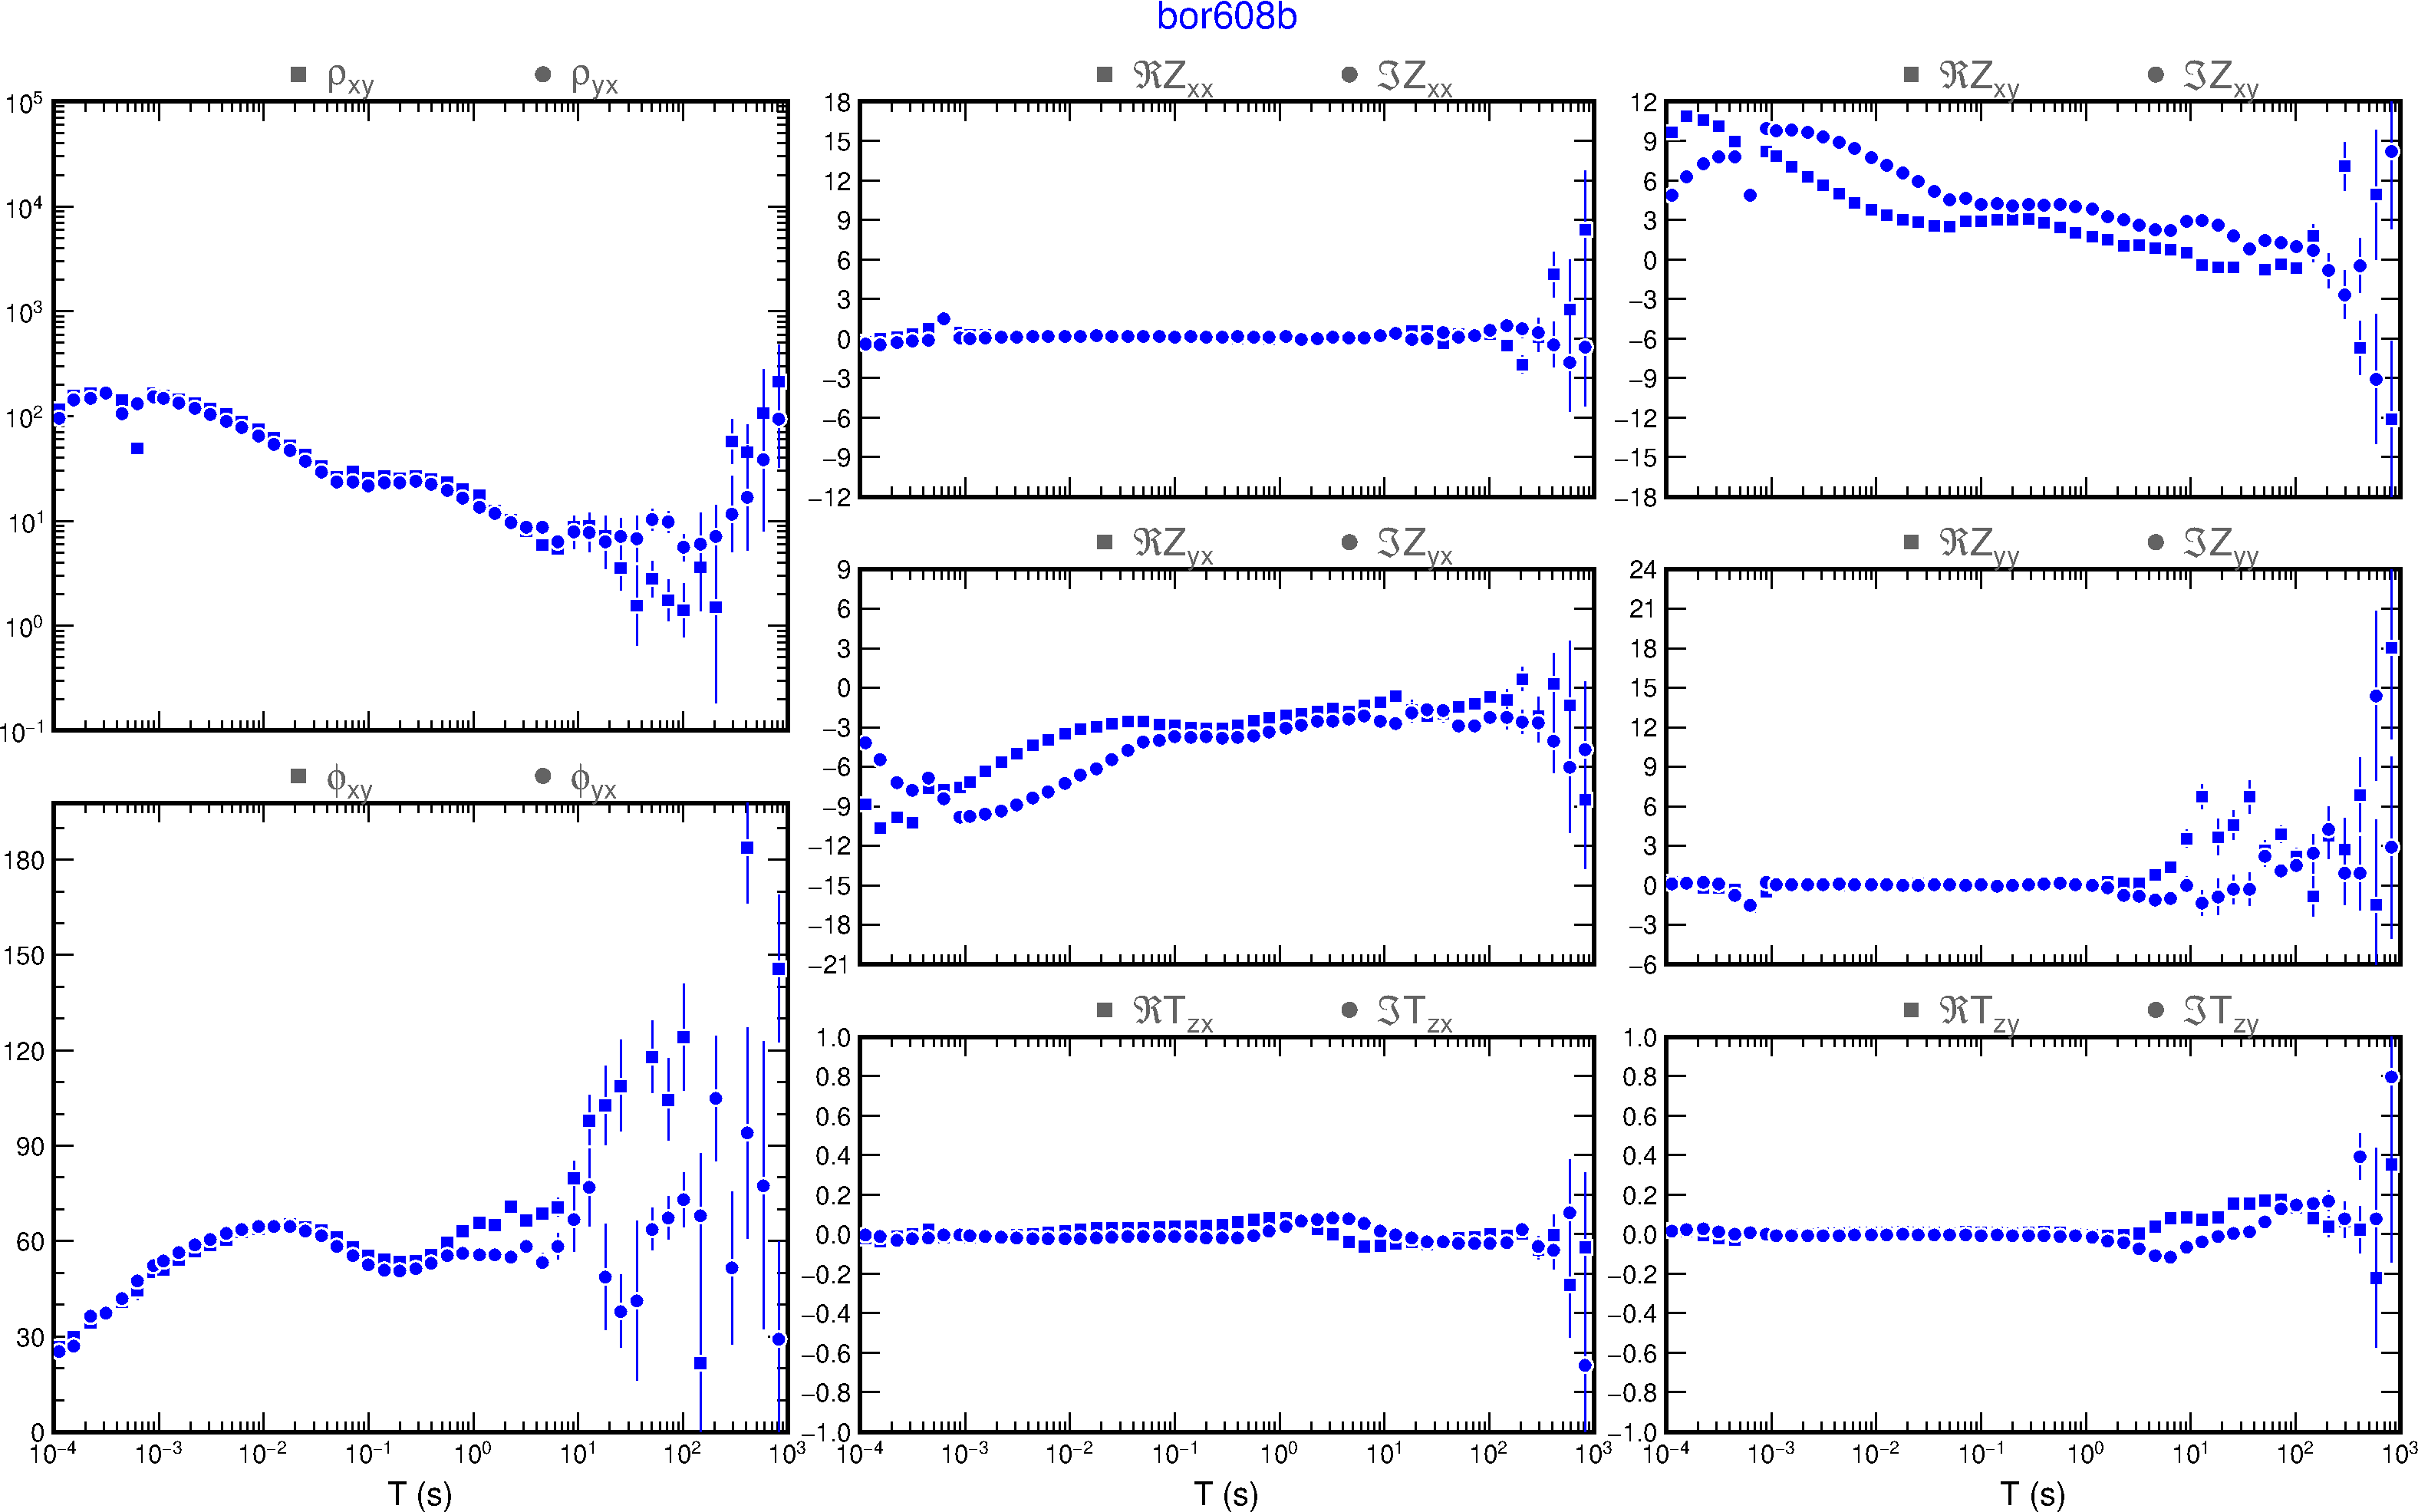
\includegraphics[width=15cm]{texto/figura/plot-cmp-tf.png}
                \end{center}
            \legend{\Fonte{\oautor.}}
            \label{plot-cmp-tf}
        \end{figure}

    
    \section{Construtor Gráfico -- Kivy}

        Kivy é um \en{framework} desenvolvido em Python com trechos escritos em Cython\footnote{Linguagem que permite  a conversão de códigos escritos com a mesma sintaxe do Python para códigos nativos em C \cite{cython}}, utilizado para o desenvolvimento da interface gráfica do programa \cite{kivy}.
        
        Kivy é um construtor gráfico que utiliza a API OpenGL \cite{opengl} para o processamento dos elementos visuais impressos na tela. Isso significa que todo o processamento dos elementos são executados nativamente no chip gráfico do computador.
        
        A escolha do Kivy também pode ser explicada pela simplicidade de implementação, visto que o mesmo permite o desenvolvimento através de uma linguagem própria, a \en{Kvlang} \cite{kvlang}. Essa linguagem permite a construção dos elementos, através de uma linguagem de marcação e indentada, ou seja, a hierarquia dos elementos estão sempre na identação mais a direita. A linguagem \en{Kvlang} é integrada ao código Python, isso permite o acesso do mesmo elemento nas duas estruturas de código.
